\chapter{Introduction}
\label{cha:introduction}

This chapter introduces the concepts of allostery in proteins, the protein structural ensemble, normal mode analysis, structural prediction of allostery, protein kinases and cyclin-dependent kinase 2 (CDK2).
% Change this to fit flow
Some of this introduction has been written as a review (cite).


\section{Allostery and the protein ensemble}


\section{Ensemble generation}

Proteins move on a variety of timescales, encompassing motions from the vibration of a single bond to the collective movement of whole domains \cite{Henzler-Wildman2007, Wei2016}.
X-ray crystallography provides a static view of the structure of proteins.
However, when only static structures are available the dynamic processes crucial to protein function \cite{Henzler-Wildman2007b} are hard to elucidate.
Experimental techniques to explore the dynamics of proteins, such as nuclear magnetic resonance (NMR), are sophisticated and time-consuming.
Molecular dynamics (MD) is a widespread computational method for predicting protein motions and generating ensembles of protein structures.
It is effective at modelling motions up to the timescale of nanoseconds.
However, the computational cost of modelling proteins on the scale of microseconds or milliseconds means MD is not suitable for larger-scale transitions.
Advanced MD methods such as targeted or accelerated MD can overcome this sampling problem \cite{Maximova2016}, but these methods are not yet routinely applicable due to the parameterisation required for each protein.

Various non-MD methods have been used to generate ensembles of protein structures from a crystal input structure, and hence explore protein dynamics.
These ensembles have uses in flexible ligand docking \cite{Totrov2008}, generating poses for protein-protein docking \cite{Mustard2005}, predicting structures on trajectories between two crystal structures \cite{Weiss2009}, and predicting flexible regions in proteins \cite{Ahmed2011}.

CONCOORD \cite{DeGroot1997, DeGroot1999} is a distance geometry method to generate structures from an input structure and consists of a two-step process.
First, the different types of chemical interactions in the input structure, e.g.\ H-bonding and hydrophobic interactions, are converted to distance constraints with a given tolerance.
Next, an iterative minimisation procedure is performed to move a set of randomly-placed coordinates such that most distance constraints are satisfied.
This generates a protein structure in a similar manner to the way a structure is produced from NMR constraints.
The process is repeated to obtain an ensemble of structures.
tCONCOORD extends CONCOORD and gives better sampling of proteins with large conformational changes by predicting H-bonds in the structure that are liable to break \cite{Seeliger2007}.


\section{Allosteric prediction}


\section{Normal mode analysis}
% Use COSB review here

Several studies have used normal mode analysis (NMA) to model allosteric regulation \cite{Mitternacht2011, Panjkovich2012, Balabin2009, Rodgers2013, Zheng2007}.
In NMA, the structural fluctuations of a protein around an equilibrium conformation are decomposed into harmonic orthogonal modes \cite{Hayward2008}.
Each mode has all parts of the system moving sinusoidally, in phase and with the same frequency.
All observed configurations of the system can be generated from a linear combination of its normal modes.
The normal modes are found by diagonalising the Hessian matrix - the matrix of second derivatives of the potential energy with respect to the mass-weighted atomic coordinates.
NMA is effective at describing protein dynamics, despite ignoring the complex nature of the protein energy landscape \cite{Bahar2005}.
Even considering the C-alpha atoms alone as a network of balls and springs can be sufficient, meaning NMA is a computationally efficient way of exploring protein flexibility compared to MD.
The long-range nature of allosteric communication is often well-described by low-frequency modes that involve the motion of many atoms.
However, allostery does involve local effects so higher-frequency modes should also be taken into account \cite{Collier2013}.
Drawback is assumes harmonic...
NMA can also be used to generate conformations of proteins, usually by modelling the protein along the relevant vibrations.
The NMSim web server \cite{Kruger2012, Ahmed2011} finds flexible and rigid protein regions using the graph theoretical approach FIRST \cite{Jacobs2001}, then generates conformations along low-frequency normal modes.
This gives sampling similar to MD but is more computationally efficient.
% Rep of above


\section{Protein kinases}

Protein kinases regulate almost all aspects of cellular physiology, from proliferation and generation of biomass to gene expression and protein production \cite{Manning2002}.
In addition to medical benefits, regulation of kinase activity in mammalian cells is important in industrial production of biomolecules of high value, for example to prevent apoptosis and maximise yield.
In order to modulate kinase activity we need to develop specific regulators of protein kinase function, a process that is complicated by the conserved catalytic architecture of the huge range of protein kinases found in nature \cite{Muller2015}.
One way to achieve kinase regulation with enhanced selectivity is through isolation of allosteric regulators, as their target sites are likely to be less structurally conserved across the protein kinase family.

A few notable examples have highlighted this potential \cite{Gavrin2013}.
Serine/threonine-protein kinase Chk1 has been the target of high-throughput screening efforts \cite{Converso2009}, leading to the discovery of an inhibitor that binds 13 \AA\ from the active site.
This inhibitor binds largely to the protein surface, with part sliding into a narrow hydrophobic cleft, indicating that unexpected sites on proteins may reveal allosteric properties.
Despite locating the allosteric binding site, the mechanism for inhibition is not currently known \cite{Vanderpool2009}.
Study of the tyrosine-protein kinase Abl1 has revealed an inhibitor that binds far from the ATP binding site \cite{Zhang2010, Yang2011}.
Binding of the modulator leads to changes in structural dynamics at the ATP binding site, preventing the binding of ATP and leading to inhibition.
Other targets for which allosteric modulators have been discovered include the MAP kinases \cite{Comess2011} and CDK2 \cite{Betzi2011}.
Modulators such as these that bind protein kinases at sites removed from the ATP-binding site are known as type IV inhibitors.
The binding sites of the above type IV inhibitors, along with others, are shown on the conserved protein kinase structure in Figure~\ref{fig:kinase_mods}.
Type I inhibitors are directly-competitive with ATP as they target the active conformation.
Type II inhibitors bind to the DFG-out conformation and occupy the ATP-binding site and the surrounding hydrophobic region.
Type III inhibitors bind the hydrophobic cleft adjacent to the ATP-binding site but do not bind the ATP-binding site itself.
A novel class of inhibitors, the type V bisubstrate and bivalent inhibitors, has emerged recently \cite{Lamba2012}.
For example, a bivalent inhibitor was designed for a tyrosine kinase that binds to the ATP-binding site and to the regulatory domain SH3 simultaneously via a linker \cite{Hill2009}.
Such binding is able to have both high selectivity and high affinity.
The recent discovery of such sites and the conserved architecture of the eukaryotic protein kinases suggest there are many allosteric sites, particularly for type IV and type V inhibitors, yet to be discovered.

Numerous examples of allosteric kinases are listed in the AlloSteric Database (ASD) \cite{Shen2016}, a resource set up in 2011 that now contains over 1,400 allosteric proteins and over 70,000 allosteric modulators.
The allosteric proteins in the ASD are those that have experimental evidence for allostery.
The increasing number of entries in this database shows that a large number of proteins have allosteric character, and implies that many proteins have allosteric character yet to be discovered.


\begin{figure}
\centering

\includegraphics[width=\textwidth]{images/kinase_mods}

\caption{Binding sites of known type IV allosteric inhibitors are shown in purple on the cAMP-dependent protein kinase (PKA) structure (PDB ID 1ATP).
The ATP binding site is shown in yellow.
Figure reproduced from Lamba and Ghosh (2012) \cite{Lamba2012}.}

\label{fig:kinase_mods}
\end{figure}


\section{Cyclin-dependent kinase 2}
% Look at Mendeley tag cdk2

CDK2 is a protein kinase important in regulating cell cycle progression \cite{Peyressatre2015}.
Its deregulation has been linked to a number of diseases.
CDK2 associates with, and is regulated by, the cyclin proteins.
The G1 to S phase checkpoint of the cell cycle is largely controlled by the CDK2-cyclin A complex.
This complex therefore is a major target of drug discovery efforts to arrest or recover control of the cell cycle in dividing cells \cite{Betzi2011}.
The mechanism of activation of CDK2 by cyclin A has been elucidated \cite{Jeffrey1995}.
Changes in the PSTAIRE helix realign active site residues, and the T-loop moves which reveals the active site and makes activation phosphorylation easier.

No CDK2 inhibitors are currently approved for clinical use.
% Check this is still true
This is due to the high conservation of the ATP-binding site among protein kinases, making a discovery of a specific CDK2 inhibitor that targets this site challenging.
It has been found that the fluorophore ANS binds at a site removed from the ATP-binding site \cite{Betzi2011}.
A screening study against this site revealed compounds that bind with affinity up to the micromolar range \cite{Rastelli2014}.
Binding of these compounds does not affect ATP binding and appears to inhibit the action of CDK2, indicating a likely allosteric site.
% Check this
